\section{Introduction} \label{sec:intro}

Introduce problem and a running example to use throughout the paper. 
clarify why we need to solve this problem.

Challenges:
\begin{itemize}
\item The number of possible \spath candidates to add to the cache are $|V|^2$. $|V|$ is the number of vertices in a road network.
\item Searching the cache must be faster than calculating a \spathns.
\item Needs to use small amount of space to achieve a good cache hit ratio.
\item How to determine the value of a path and all its possible subpaths.
\end{itemize}


\begin{figure}
  \center
        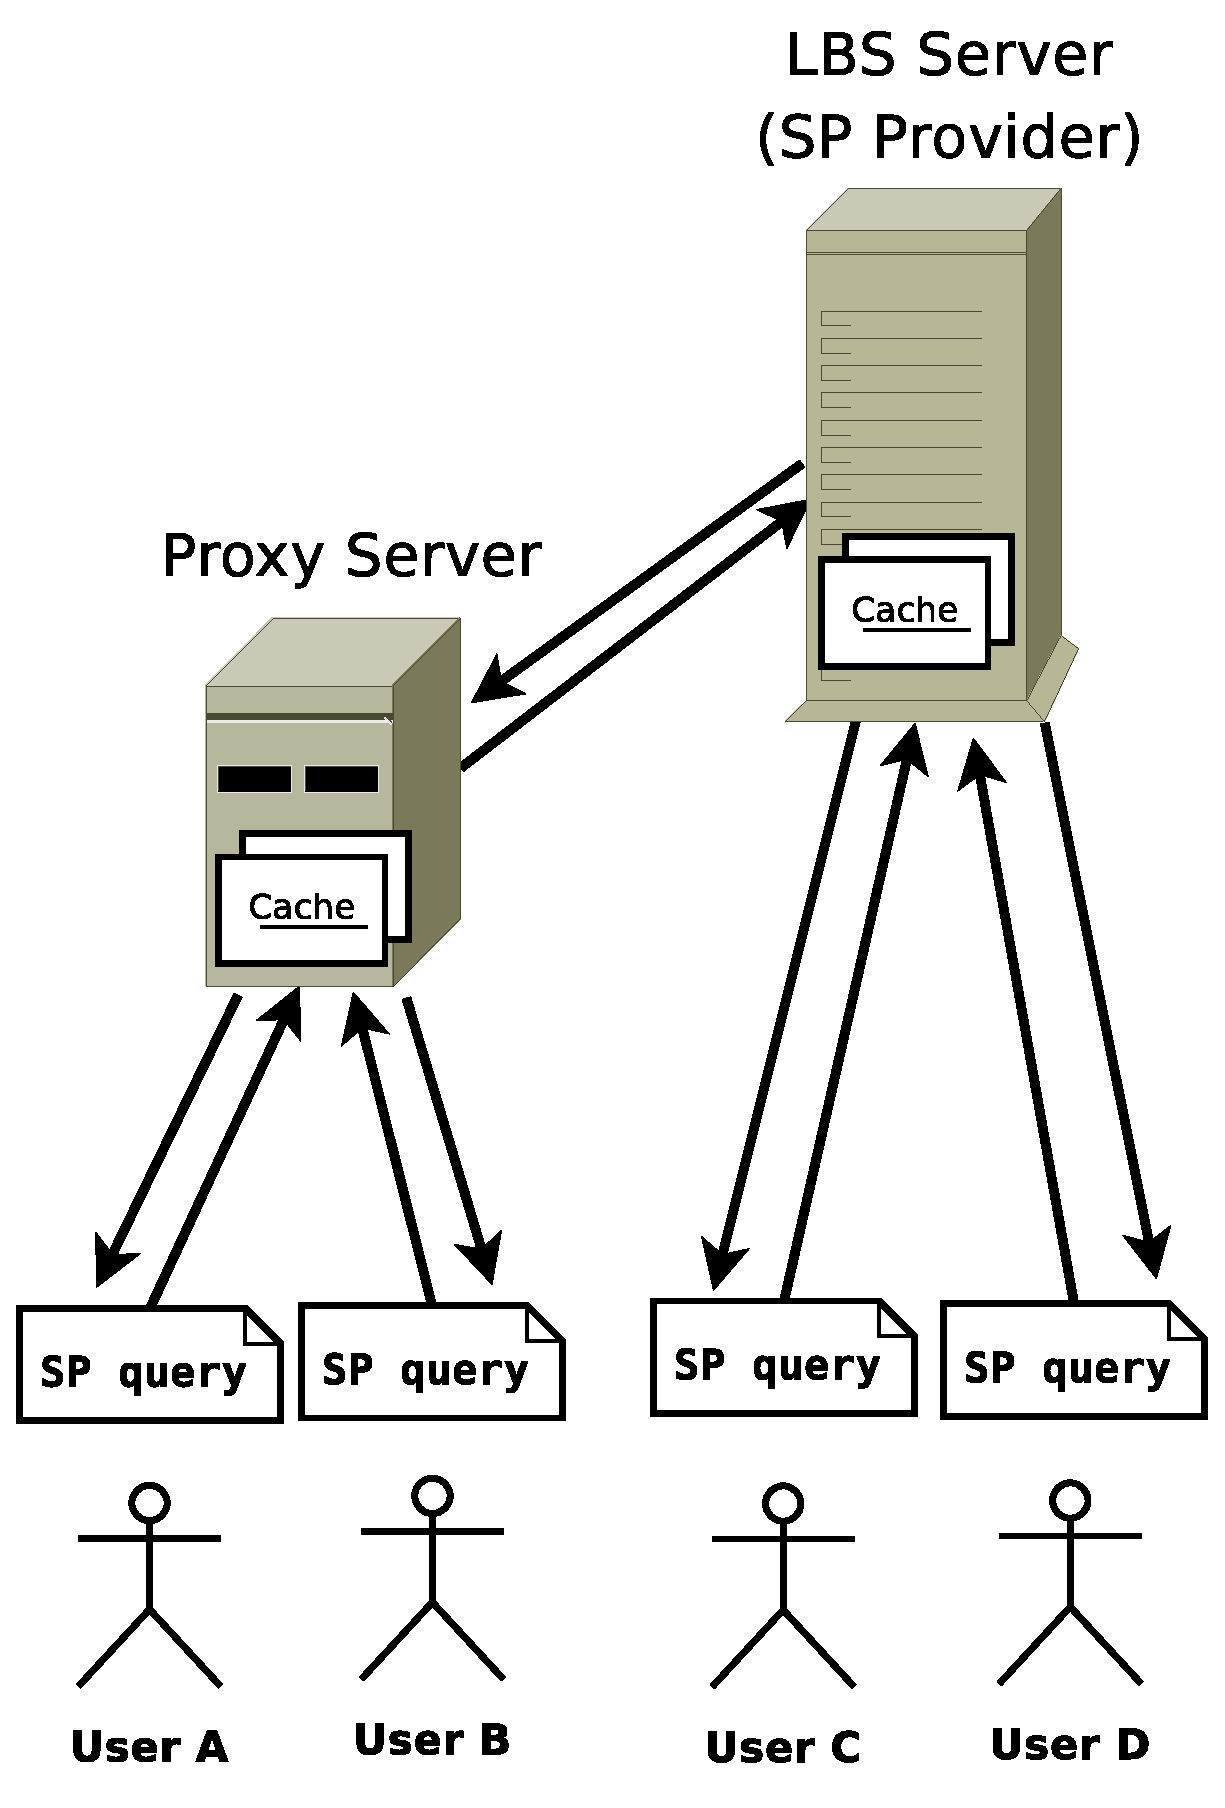
\includegraphics[width=0.25\textwidth]{figures/scenario}
        \caption{Overall scenario showing where the cache could be placed and where users may submit \spath queries.}
  \label{fig:routequery}
\end{figure}